\section{Présentation de l'entreprise}

\subsection{Histoire}
Orange Cyberdefense est une entreprise française leader européen de la cybersécurité, proposant des services de protection, de détection et de réponse aux cybermenaces. L'entreprise s'est construite progressivement à partir des expertises en sécurité du groupe Orange, avant de connaître une accélération majeure avec des acquisitions stratégiques.

Les premières activités de cybersécurité d'Orange remontent aux années 2000, lorsque l'opérateur développe ses capacités internes de protection des infrastructures et des données. En 2016, Orange structure officiellement sa division cybersécurité sous la marque Orange Cyberdefense.

L'année 2019 marque un tournant décisif avec l'acquisition de Securelink, leader européen des services managés de cybersécurité. Cette opération permet à Orange Cyberdefense de devenir l'un des principaux acteurs européens du secteur, en intégrant plus de 1 000 experts en sécurité.

Orange Cyberdefense connaît une croissance soutenue avec une expansion internationale continue. L'entreprise compte aujourd'hui plus de 3 000 experts répartis dans plus de 20 pays et protège plus de 2 000 organisations à travers le monde.

La figure suivante montre la présence de l’entreprise dans le monde 

\begin{figure}[H]
\centering
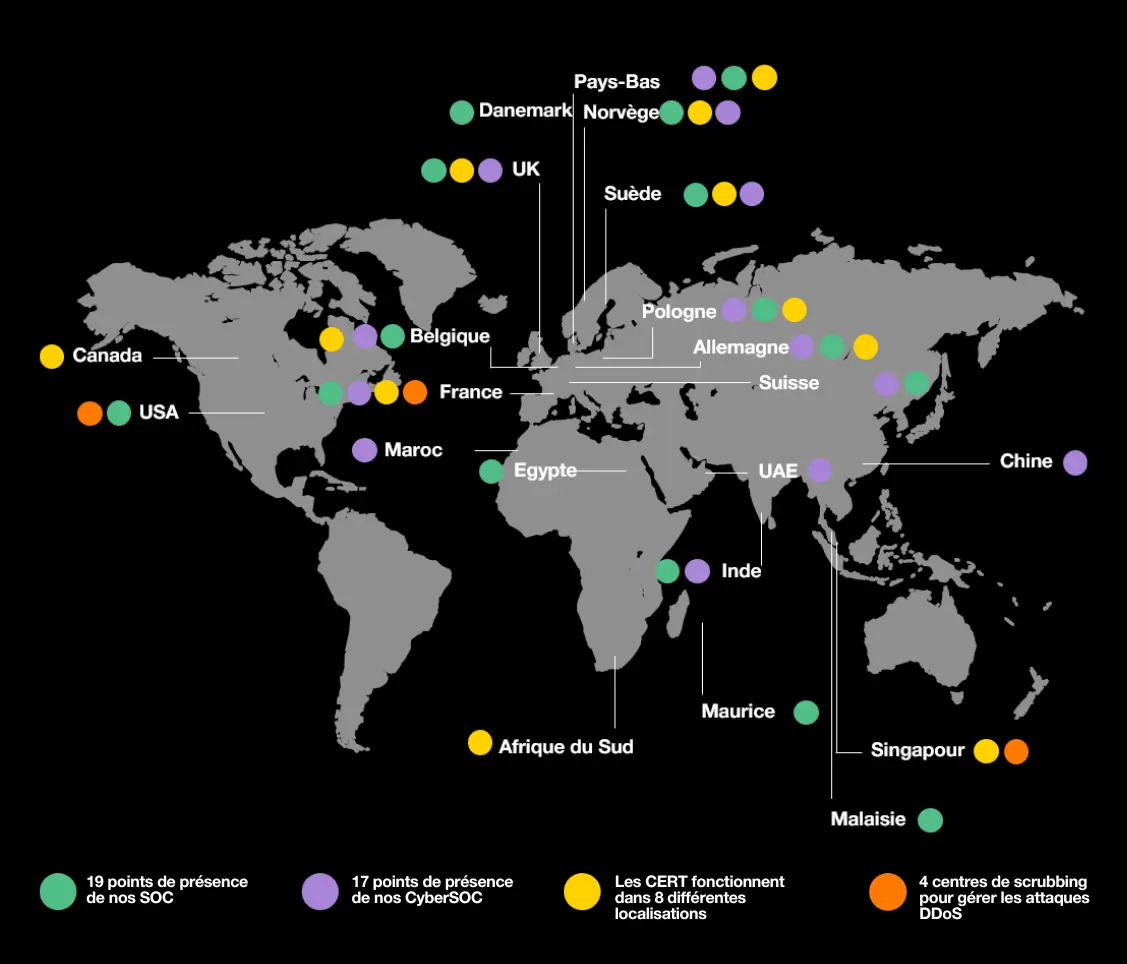
\includegraphics[width=0.7\textwidth]{assets/OCD_world.png}
\caption{Présence d'Orange Cyberdefense dans le monde}
\end{figure}

\subsection{Services et Produits}
L'entreprise structure son offre autour du cycle de vie complet de la cybersécurité : anticiper, identifier, protéger, détecter et répondre. Elle propose ainsi des services de conseil et gestion des risques, d'audit et tests d'intrusion, de détection et réponse aux incidents via un réseau mondial de SOC, ainsi que de gestion des vulnérabilités.\footnote{L'entreprise propose un large gamme de services en cybersécurité. Dans le cadre de cette alternance, je présente uniquement les services en lien direct avec ma mission.}

\subsubsection{L'Unified Managed Firewall (UMFW)}

Parmi ces services, l'Unified Managed Firewall (UMFW) occupe une place centrale. Il s'agit d'un service managé de pare-feu, qui assure la protection en continu des réseaux des clients contre les intrusions et attaques externes. Le MFW permet de filtrer le trafic, d'appliquer des politiques de sécurité adaptées et de détecter les comportements suspects en temps réel, tout en déchargeant les équipes internes des clients de la gestion quotidienne de cette protection.

Pour couvrir les besoins variés de ses clients, Orange Cyberdefense s'appuie sur plusieurs technologies de pare-feu de référence, notamment \textit{Fortinet}, \textit{Check Point} et \textit{Palo Alto Networks}. Chaque technologie est sélectionnée selon le contexte et les exigences de l'environnement du client.

Dans ce cadre, mon alternance s'inscrit au sein de l'équipe d'expertise \textit{Check Point}, en charge de la gestion et de l'administration des solutions de pare-feu Check Point déployées chez les clients d'Orange Cyberdefense.

\subsection{Structure de l'entreprise}
TODO : mentionner que nous somme dans la 2eme BU et dnas le GOPS

TODO : mentionner qu'il y les expert et les devs dans l'équipe

TODO : mon positionnement dans l'équipe